\documentclass[10pt, titlepage]{article}

\usepackage[margin=1in]{geometry}
\usepackage{graphicx}
\usepackage{float}
\usepackage{xcolor,listings}
\usepackage[most]{tcolorbox}
\usepackage{hyperref}
\usepackage{subcaption}
\usepackage{times} % for Times New Roman font
\usepackage{setspace} % for single spacing
\parindent 0px % no indentation

\title{\textbf{ECCS 3411\\Computer Security}\\Password Manager Application}
\author{Kento Akazawa, Jada Benjamin, Grant Daly, Brian Watkins}
\date{April 28, 2024}

\hypersetup{
	colorlinks=true,
	linkcolor=blue,
	citecolor=blue,
	filecolor=magenta,  
	urlcolor=cyan,
	pdftitle={Overleaf Example},
	pdfpagemode=FullScreen,
}

\lstdefinelanguage{swift}
{
  morekeywords={
    func,if,then,else,for,in,while,do,switch,case,default,where,break,continue,fallthrough,return,
    typealias,struct,class,enum,protocol,var,func,let,get,set,willSet,didSet,inout,init,deinit,extension,
    subscript,prefix,operator,infix,postfix,precedence,associativity,left,right,none,convenience,dynamic,
    final,lazy,mutating,nonmutating,optional,override,required,static,unowned,safe,weak,internal,
    private,public,is,as,self,unsafe,dynamicType,true,false,nil,Type,Protocol,
    String,Data,UserDefaults,guard,fatalError,Bool,SymmetricKey,Password,
    NSManagedObjectContext,try,catch,print
  },
  morecomment=[l]{//}, % l is for line comment
  morecomment=[s]{/*}{*/}, % s is for start and end delimiter
  morestring=[b]" % defines that strings are enclosed in double quotes
}

\definecolor{keyword}{HTML}{BA2CA3}
\definecolor{string}{HTML}{D12F1B}
\definecolor{comment}{HTML}{008400}
\definecolor{lightgray}{HTML}{F5F5F5}

\lstset{
  language=swift,
  basicstyle=\ttfamily,
  showstringspaces=false, % lets spaces in strings appear as real spaces
  columns=fixed,
  keepspaces=true,
  numbers=left,
  numberstyle=\tiny\color{gray},
  showstringspaces=false,
  keywordstyle=\color{keyword},
  stringstyle=\color{string},
  commentstyle=\color{comment},
  backgroundcolor=\color{lightgray},
  linewidth=0.95\textwidth
}

\begin{document}
\maketitle
\newpage

\tableofcontents
\newpage

\section*{Introduction}
\addcontentsline{toc}{section}{Introduction}
In today's digital landscape, where online security is paramount, the need for robust password management solutions has never been greater. For this project, we created password manager app in Swift. It offers users a secure and convenient way to store their passwords, along with associate titles, usernames, and websites. Leveraging advanced encryption and hashing techniques, this app ensures that sensitive user data remains protected against unauthorized access and potential breaches. This project can be found \href{https://github.com/k-akzw/PasswordManager.git}{here}.

\section*{Data}
\addcontentsline{toc}{section}{Data}
Access to stored passwords is controlled by a master password, ensuring confidentiality. Each password entry is assigned a unique ID, allowing for efficient management of multiple entries with the same information. Leveraging \texttt{CoreData}, passwords are stored securely within the application's database. 

\section*{User Interface}
\addcontentsline{toc}{section}{User Interface}
When launching the app for the first time, it asks to set the master password as shown in \autoref{fig:set_pw} below. 
\begin{figure}[H]
	\centering
	\vspace{-0.25em}
	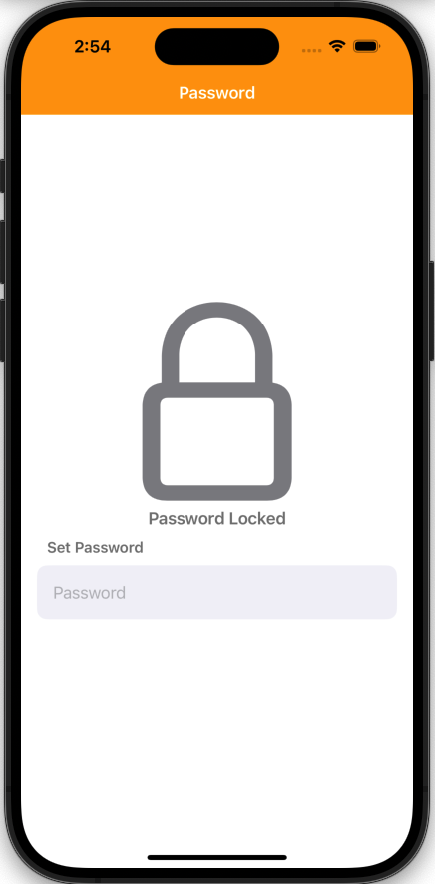
\includegraphics[width=0.4\textwidth]{img/set_pw}
	\vspace{-0.75em}
	\caption{Setting Master Password}
	\label{fig:set_pw}
	\vspace{-0.75em}
\end{figure}

Enhancing the security of our application, we implemented a robust measure by hashing the master password using the SHA-256 algorithm before storage. This one-way hashing process ensures that even in the event of a breach, the original password remains secure. The hashing function, elaborated upon later in this report, provides an additional layer of protection against unauthorized access, as it is computationally infeasible to determine original password from hashed password.

When the app launches after the master password is set, it asks for the password as shown in \autoref{fig:enter_pw}.
\begin{figure}[H]
	\centering
	\vspace{-0.25em}
	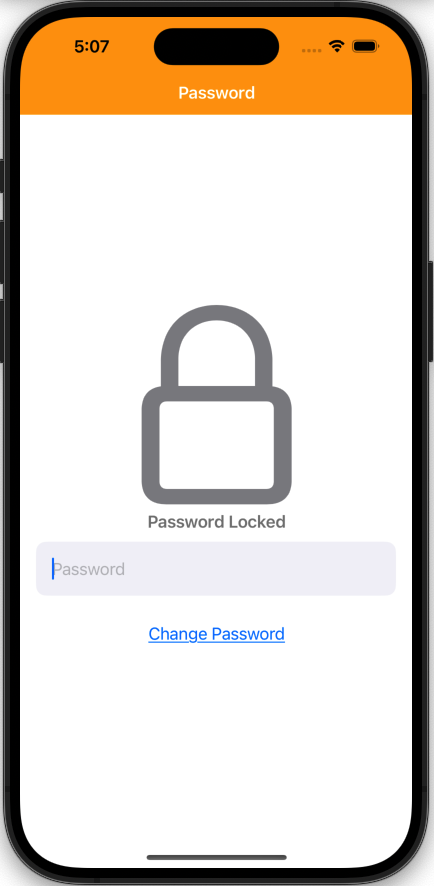
\includegraphics[width=0.3\textwidth]{img/enter_pw}
	\vspace{-0.75em}
	\caption{Entering Password}
	\label{fig:enter_pw}
	\vspace{-0.75em}
\end{figure}

The entered password will be hashed and compared with saved hashed master password. If they do not match, it displays a message showing that entered password is wrong as shown in \autoref{fig:enter_wrong_pw}. 
\begin{figure}[H]
	\centering
	\vspace{-0.25em}
	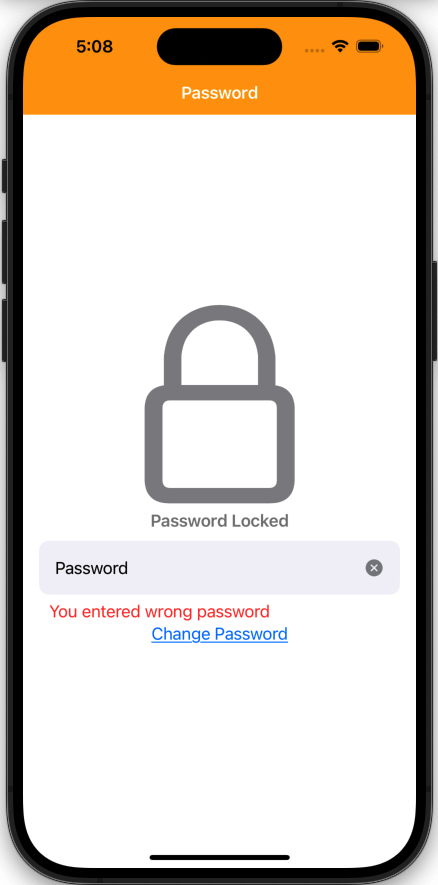
\includegraphics[width=0.3\textwidth]{img/enter_wrong_pw}
	\vspace{-0.75em}
	\caption{When wrong password is entered}
	\label{fig:enter_wrong_pw}
	\vspace{-0.75em}
\end{figure}

The password can be changed by tapping \texttt{Change Password} link. This navigates to a screen shown in \autoref{fig:change_pw}.
\begin{figure}[H]
	\centering
	\vspace{-0.25em}
	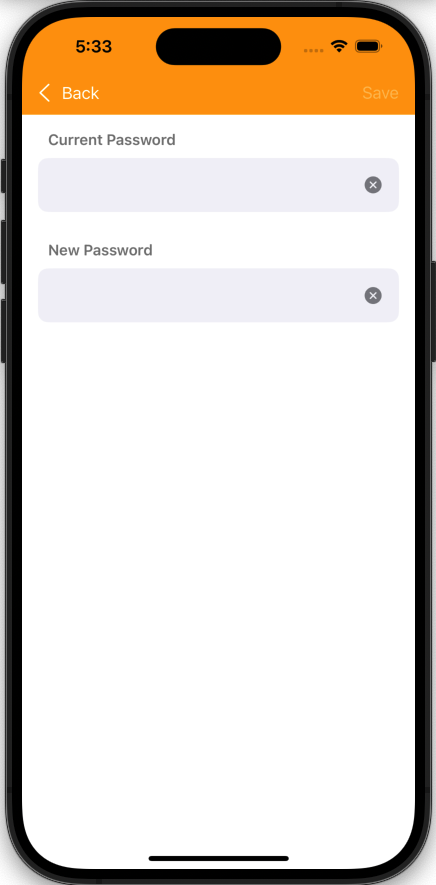
\includegraphics[width=0.3\textwidth]{img/change_pw}
	\vspace{-0.75em}
	\caption{Changing master password}
	\label{fig:change_pw}
	\vspace{-0.75em}
\end{figure}
Once current password and new password are entered, save button on the top right will be enabled. If the current password matches with the saved password, new master password will be saved and navigate back to the initial screen (\autoref{fig:enter_pw}).

If the entered password is correct in the initial screen (\autoref{fig:enter_pw}), it grants access to the list of passwords saved and displays them as shown in \autoref{fig:pw_list}.
\begin{figure}[H]
	\centering
	\vspace{-0.25em}
	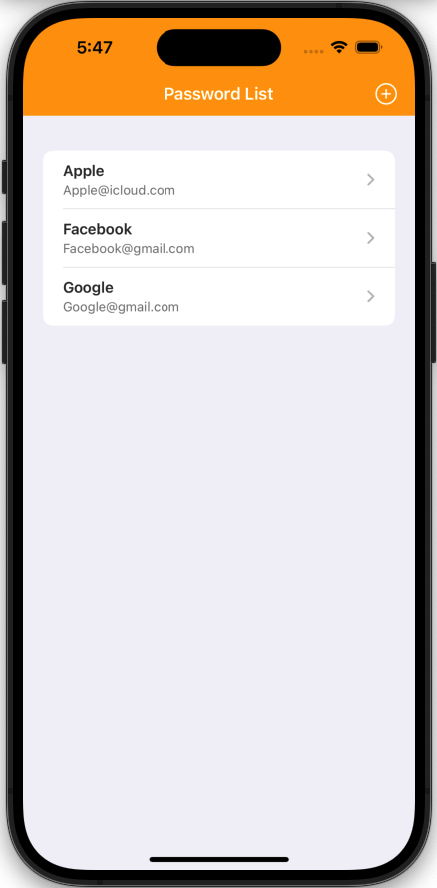
\includegraphics[width=0.3\textwidth]{img/pw_list}
	\vspace{-0.75em}
	\caption{List of saved passwords}
	\label{fig:pw_list}
	\vspace{-0.75em}
\end{figure}

New password can be added by tapping on plus symbol on the top right. It will navigate to screen shown in \autoref{fig:add_pw}.
\begin{figure}[H]
	\centering
	\vspace{-0.25em}
	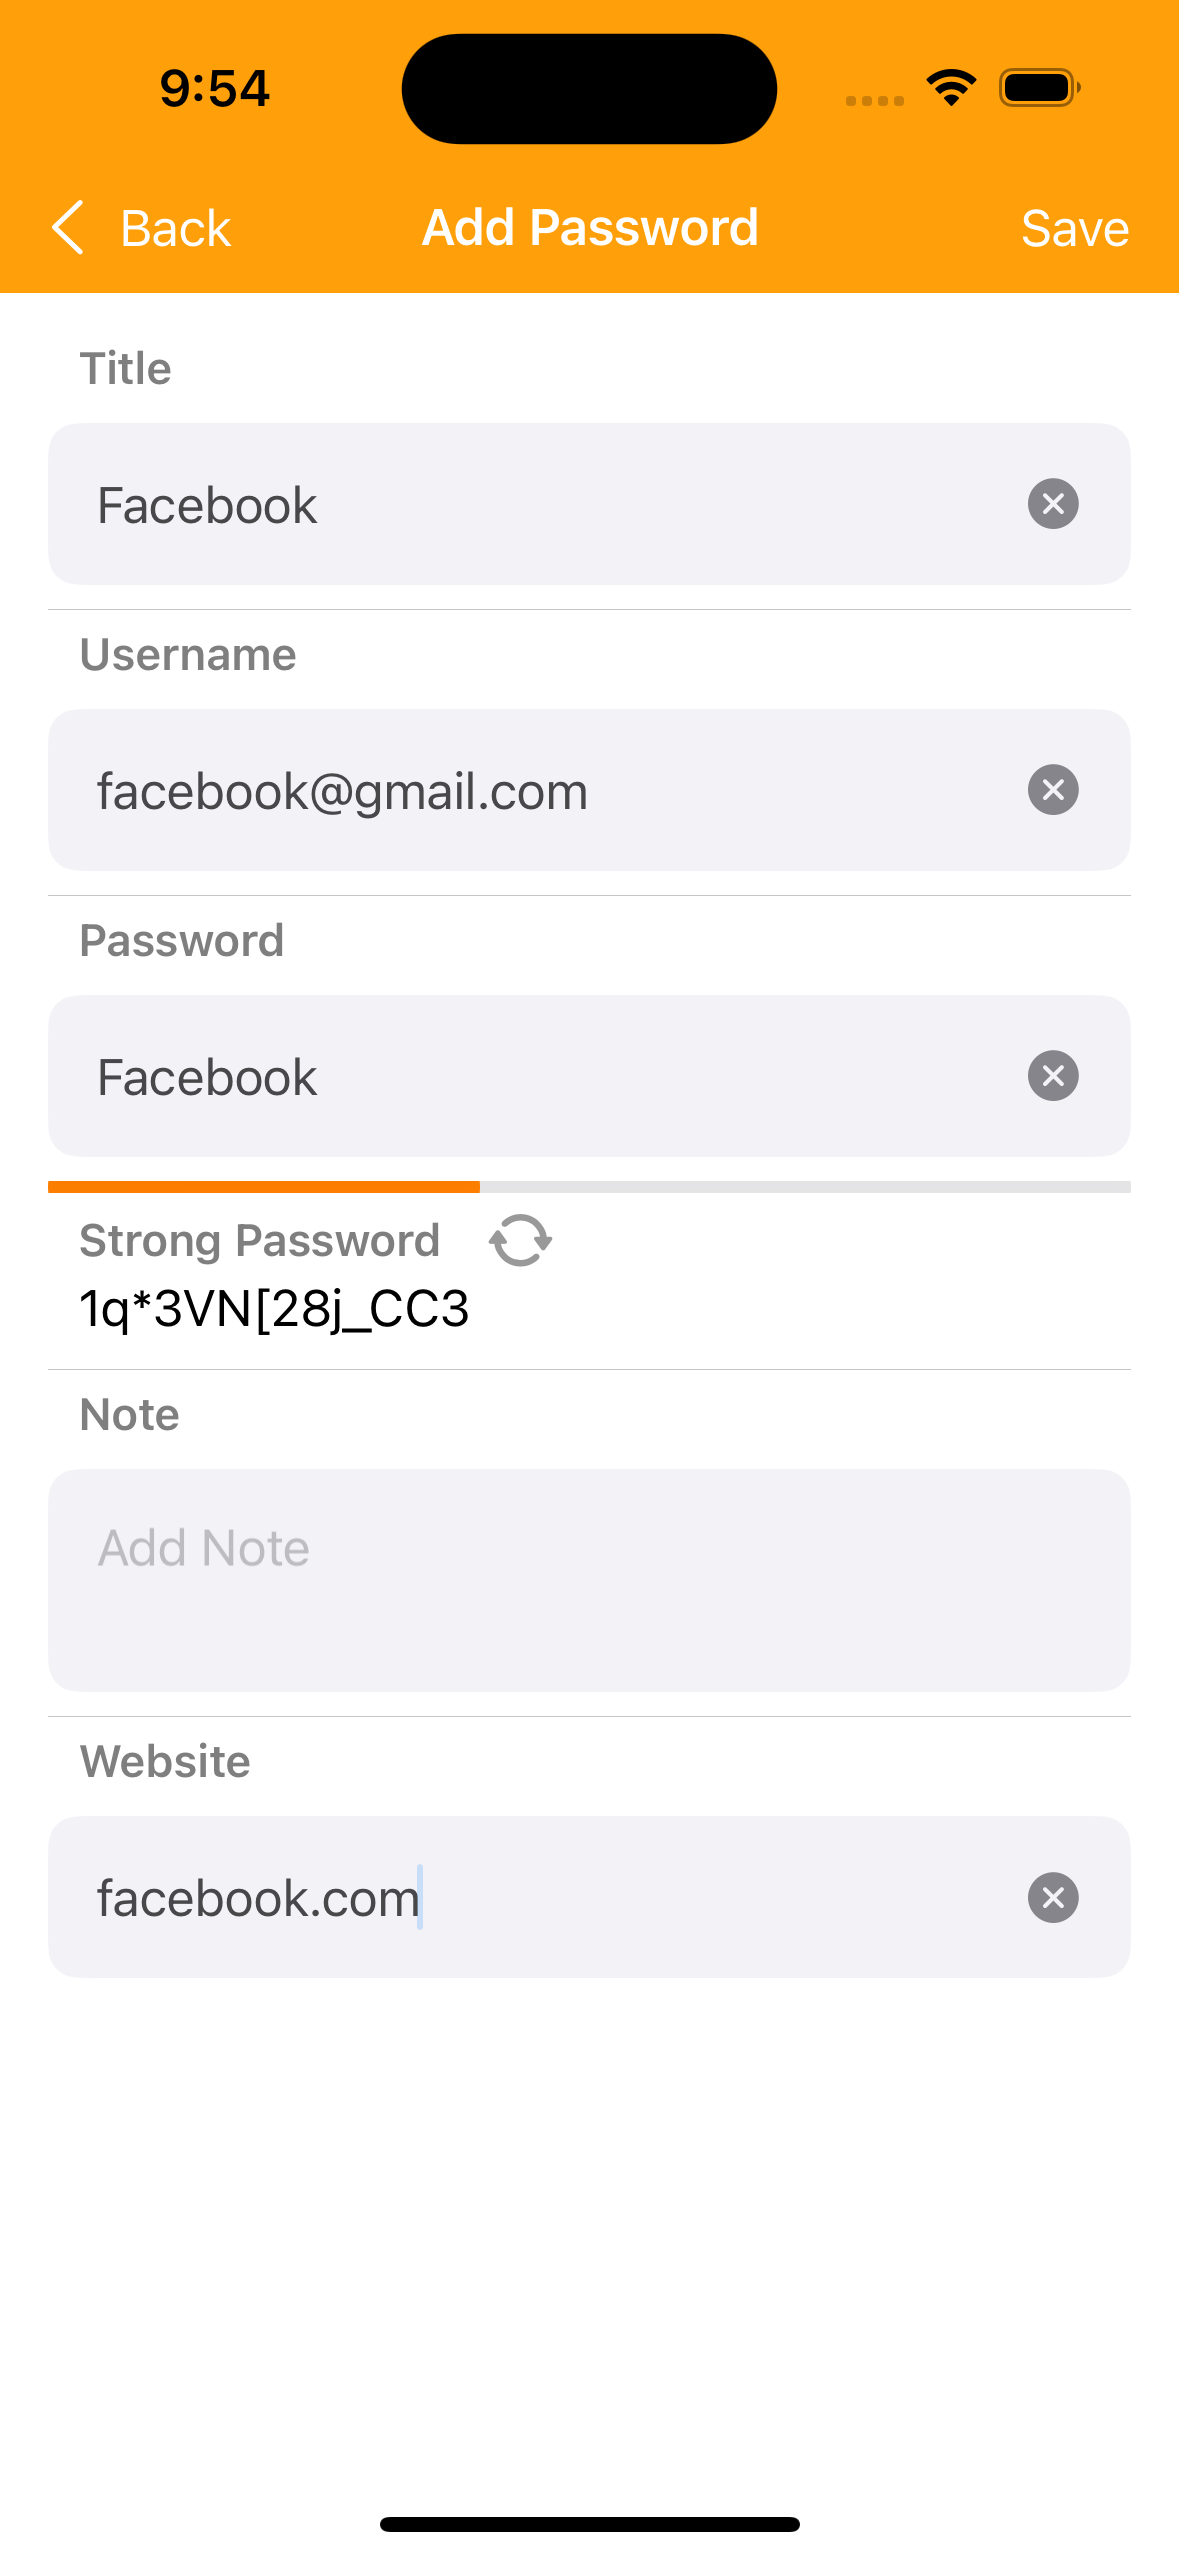
\includegraphics[width=0.3\textwidth]{img/add_pw}
	\vspace{-0.75em}
	\caption{Adding new password}
	\label{fig:add_pw}
	\vspace{-0.75em}
\end{figure}

Each password stored in our system consists of a title, username, password, note, and website. We have implemented a feature that generates robust passwords automatically and provides users with a visual password strength meter to educate them on the strength of their chosen passwords. Additionally, if a user attempts to save a weak password, an alert is displayed to warn them about its vulnerability, as illustrated in \autoref{fig:weak_alert}. This proactive approach encourages users to select stronger passwords, thereby enhancing the overall security of our application.
\begin{figure}[H]
	\centering
	\vspace{-0.25em}
	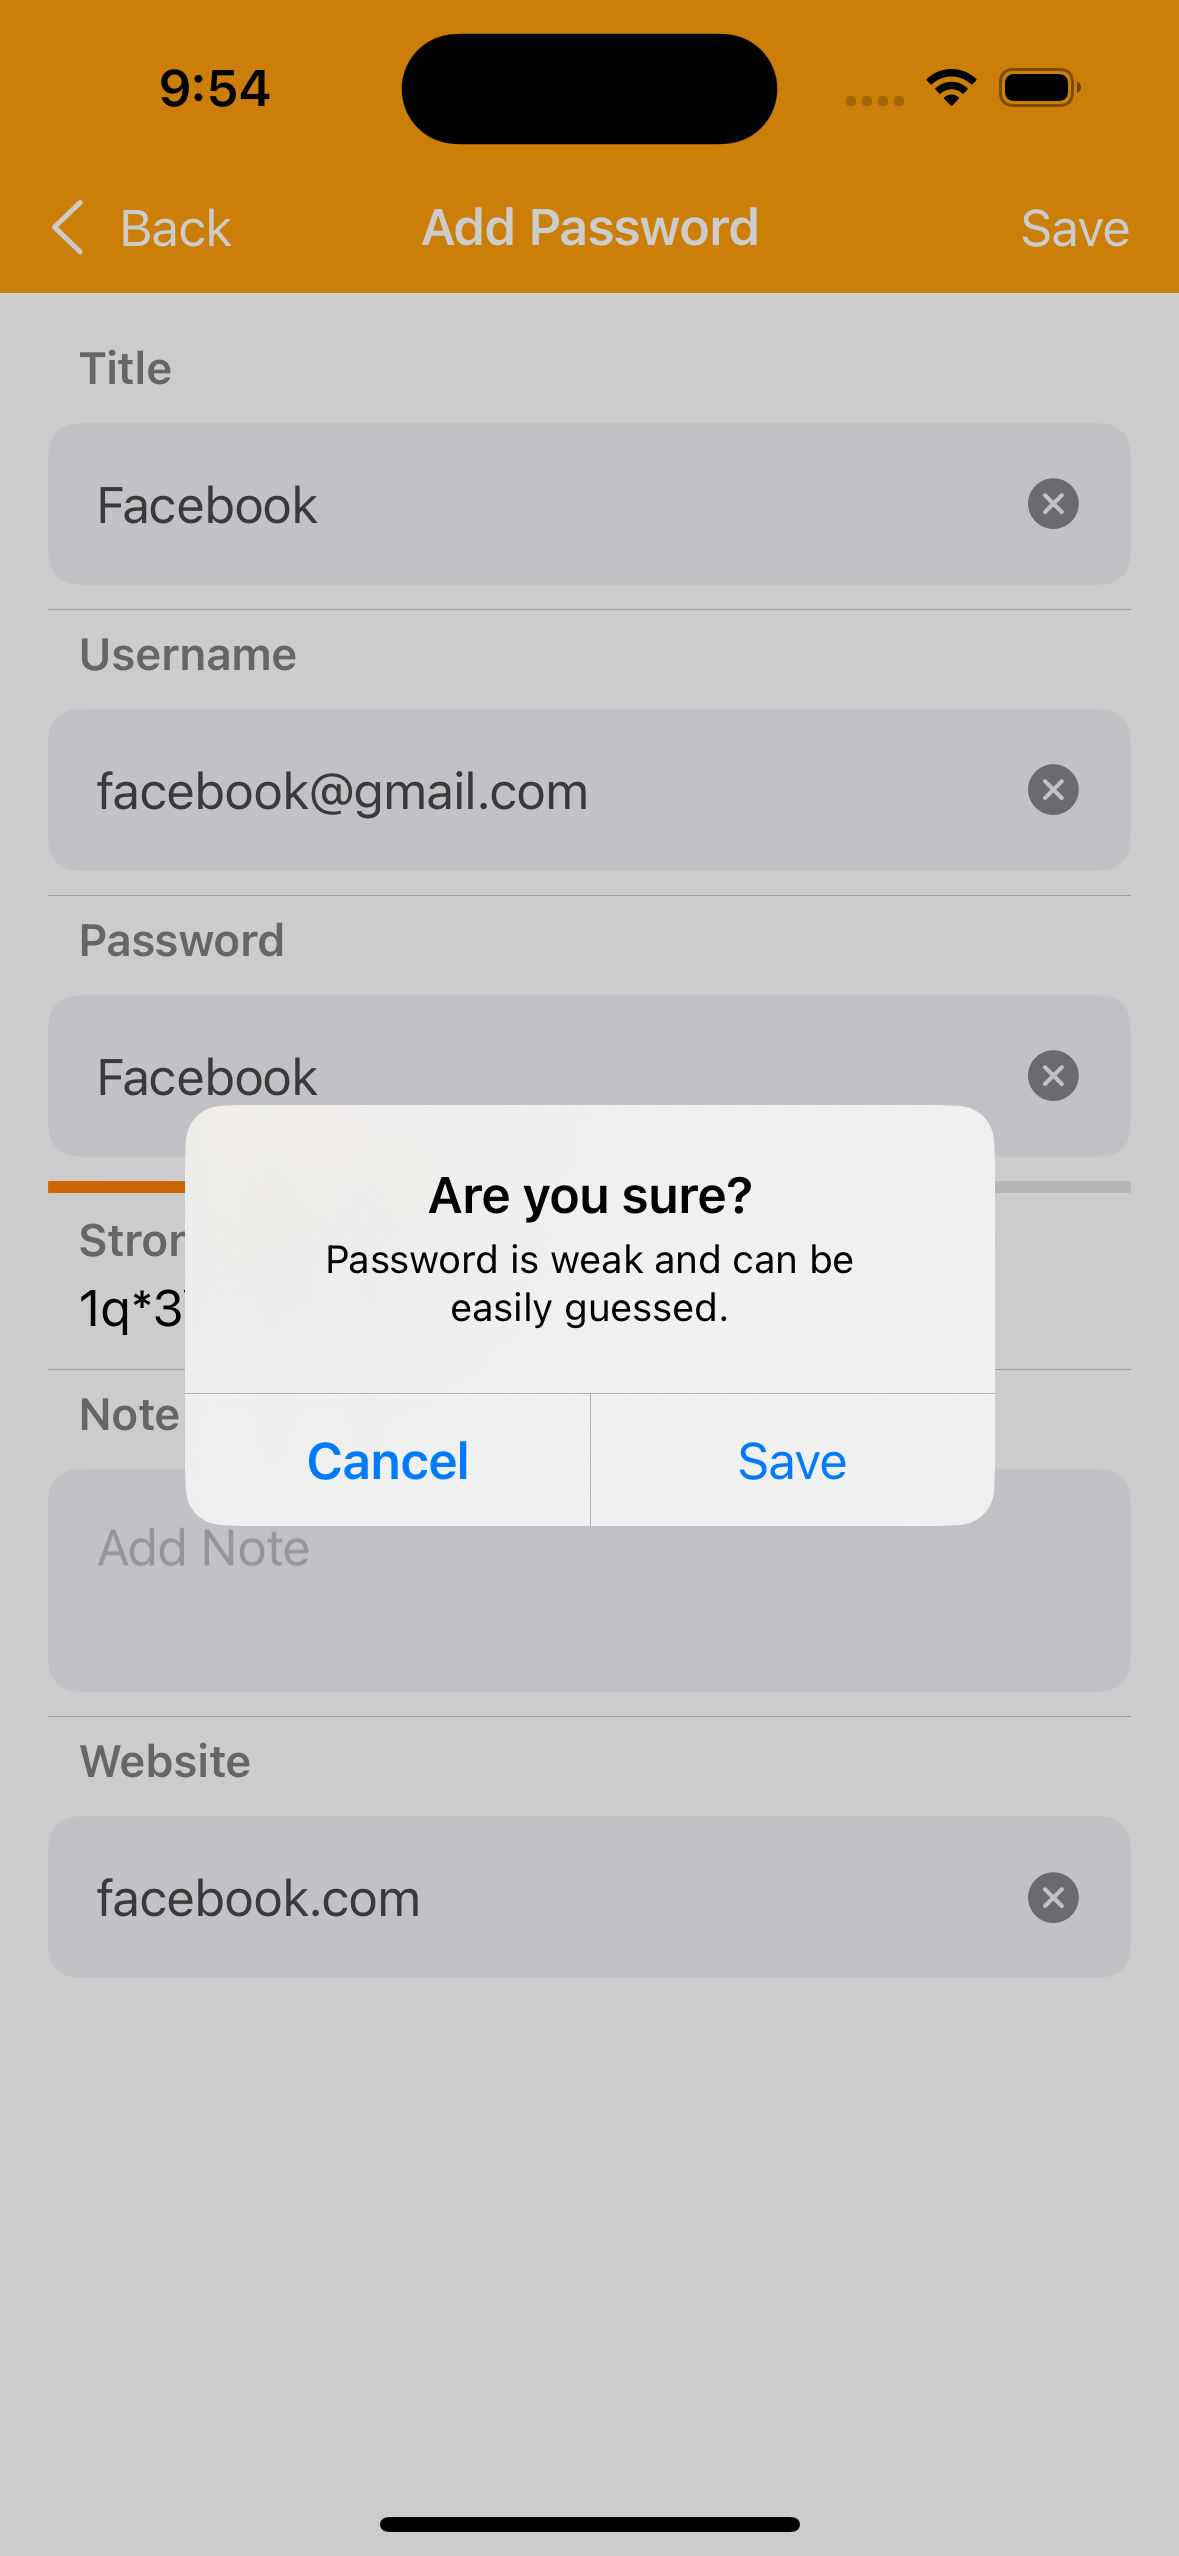
\includegraphics[width=0.3\textwidth]{img/weak_alert}
	\vspace{-0.75em}
	\caption{Alert for attempting to save weak password}
	\label{fig:weak_alert}
	\vspace{-0.75em}
\end{figure}

When users access the password list screeen (\autoref{fig:pw_list}), they are presented with the titles and usernames of their stored passwords. Upon selecting a specific entry, users are directed to the password detail screen (\autoref{fig:pw_detail_0}), where the password is initially concealed to protect against shoulder surfing. However, users can reveal the password by tapping on it, as depicted in \autoref{fig:pw_detail_1}. Each password is encrypted before storage and decrypted when launching password detail screen (\autoref{fig:pw_detail_0}). This approach balances security with usability, allowing users quick access to their passwords while maintaining confidentiality.
\begin{figure}[H]
    \centering
    \begin{subfigure}[b]{0.45\textwidth}
        \centering
        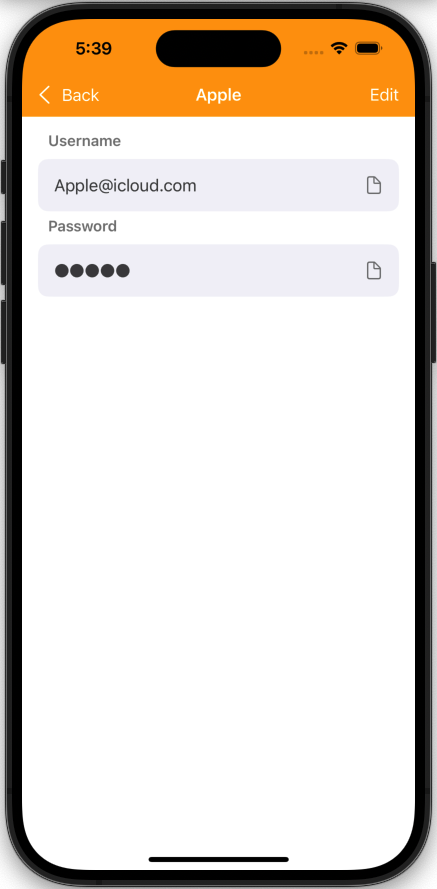
\includegraphics[width=\linewidth]{img/pw_detail_0}
        \caption{}
        \label{fig:pw_detail_0}
    \end{subfigure}\hfill
    \begin{subfigure}[b]{0.45\textwidth}
        \centering
        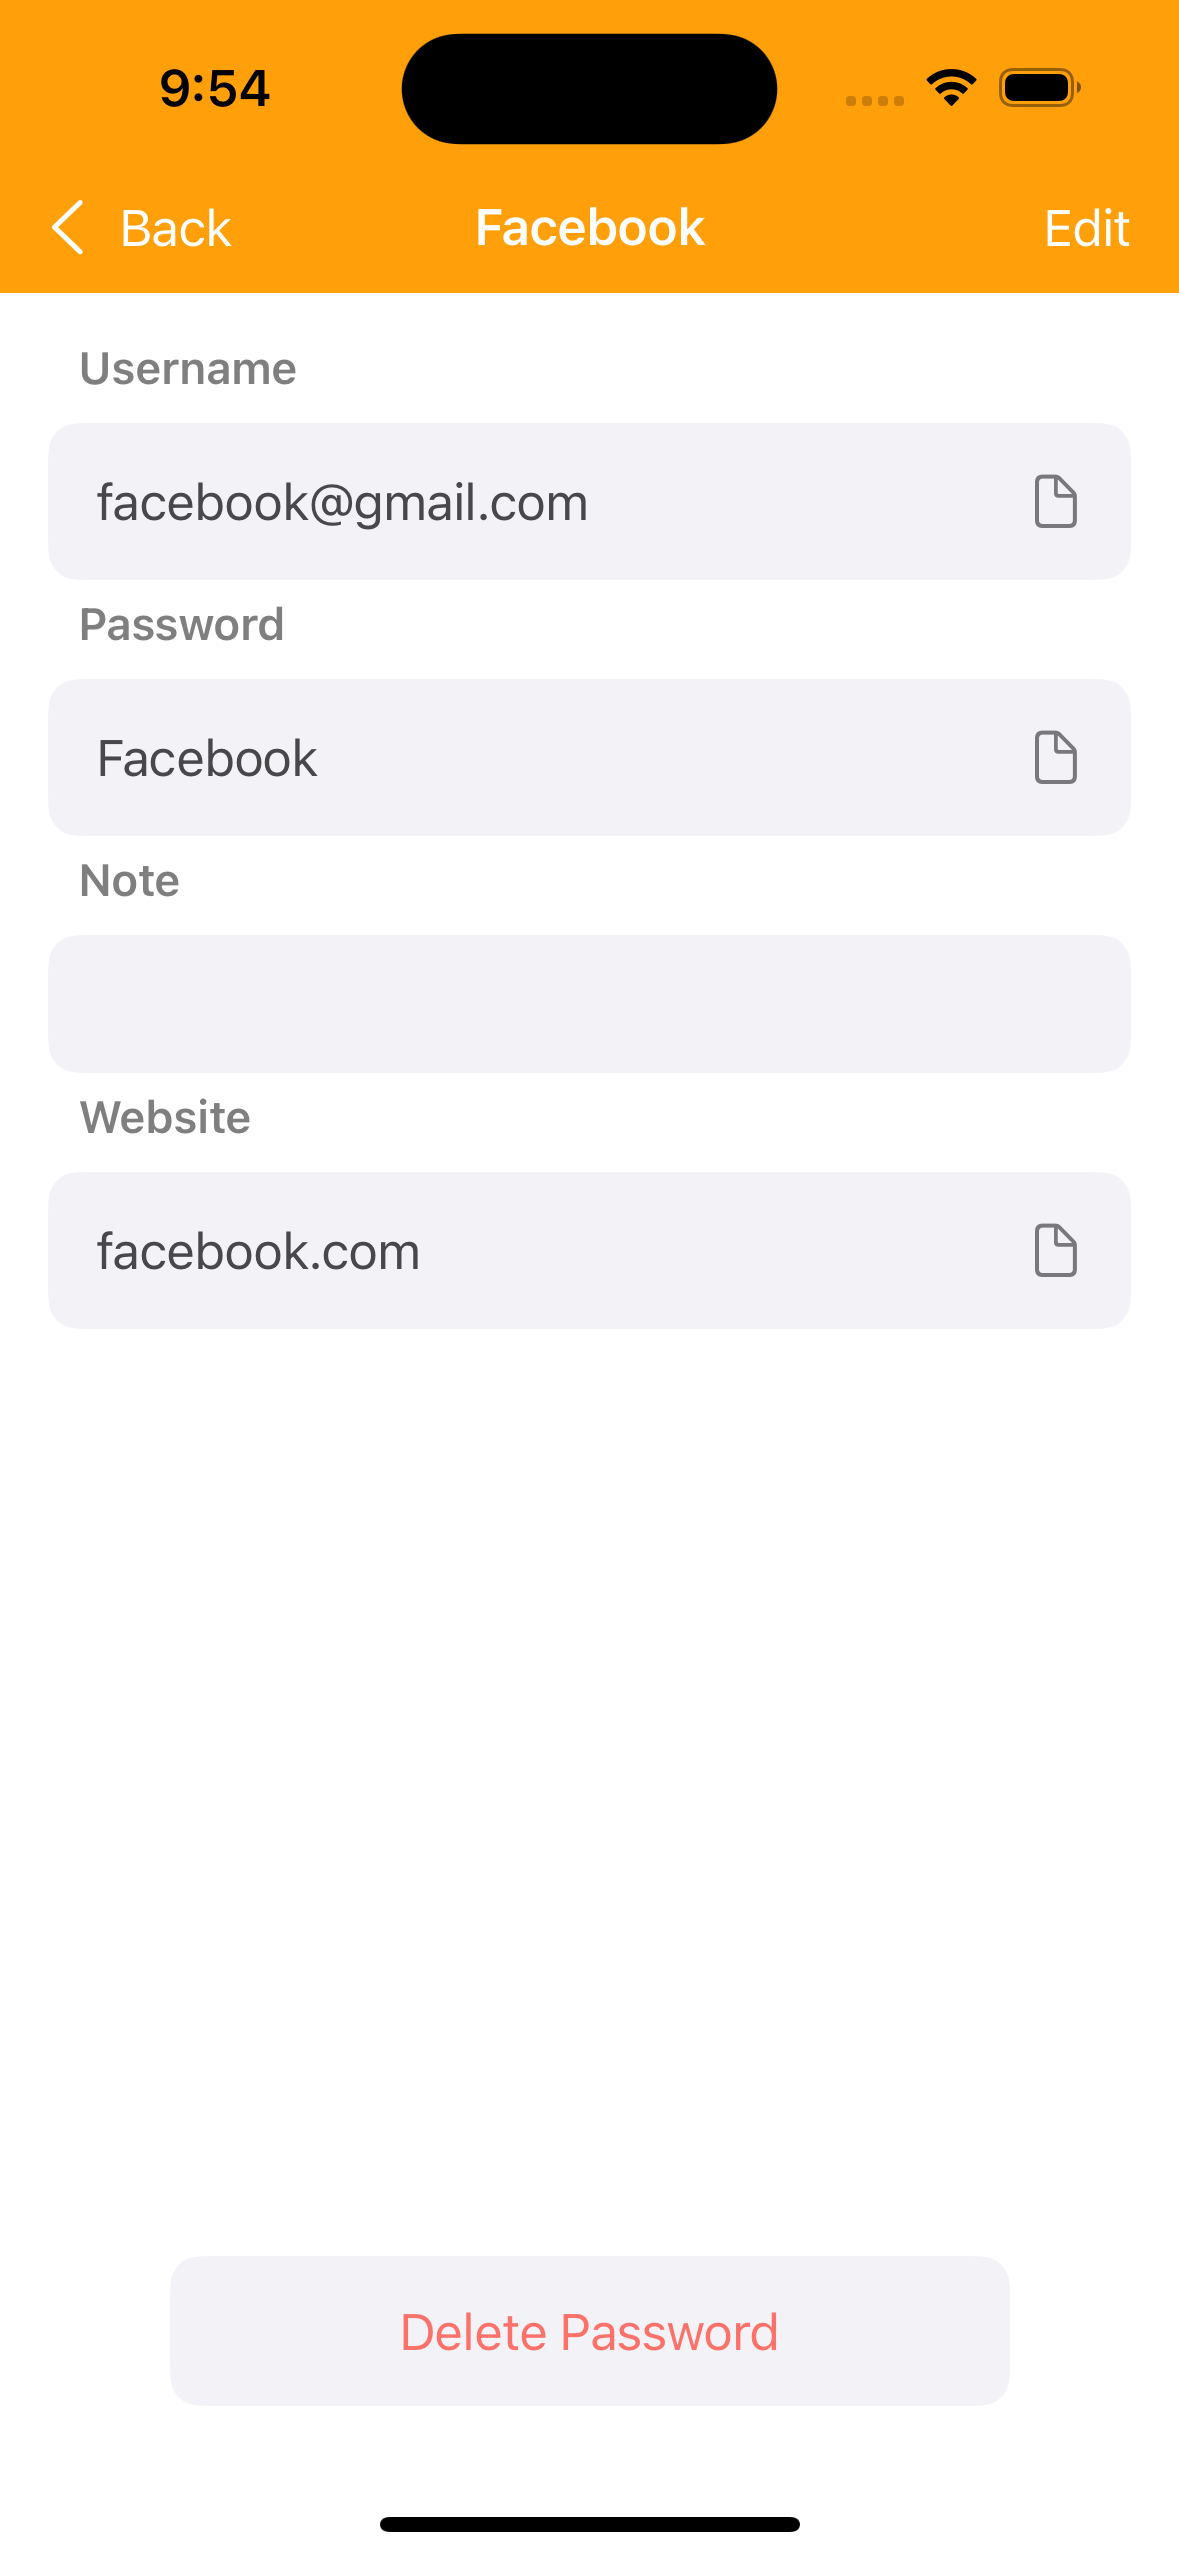
\includegraphics[width=\linewidth]{img/pw_detail_1}
        \caption{}
        \label{fig:pw_detail_1}
    \end{subfigure}
    \caption{Password detail view}
    \label{fig:pw_detail}
\end{figure}

Stored information can be modified by tapping on \texttt{Edit} button on top right of the screen (\autoref{fig:pw_detail}). This will navigate to screen show in \autoref{fig:edit_pw}. 

\begin{figure}[H]
	\centering
	\vspace{-0.25em}
	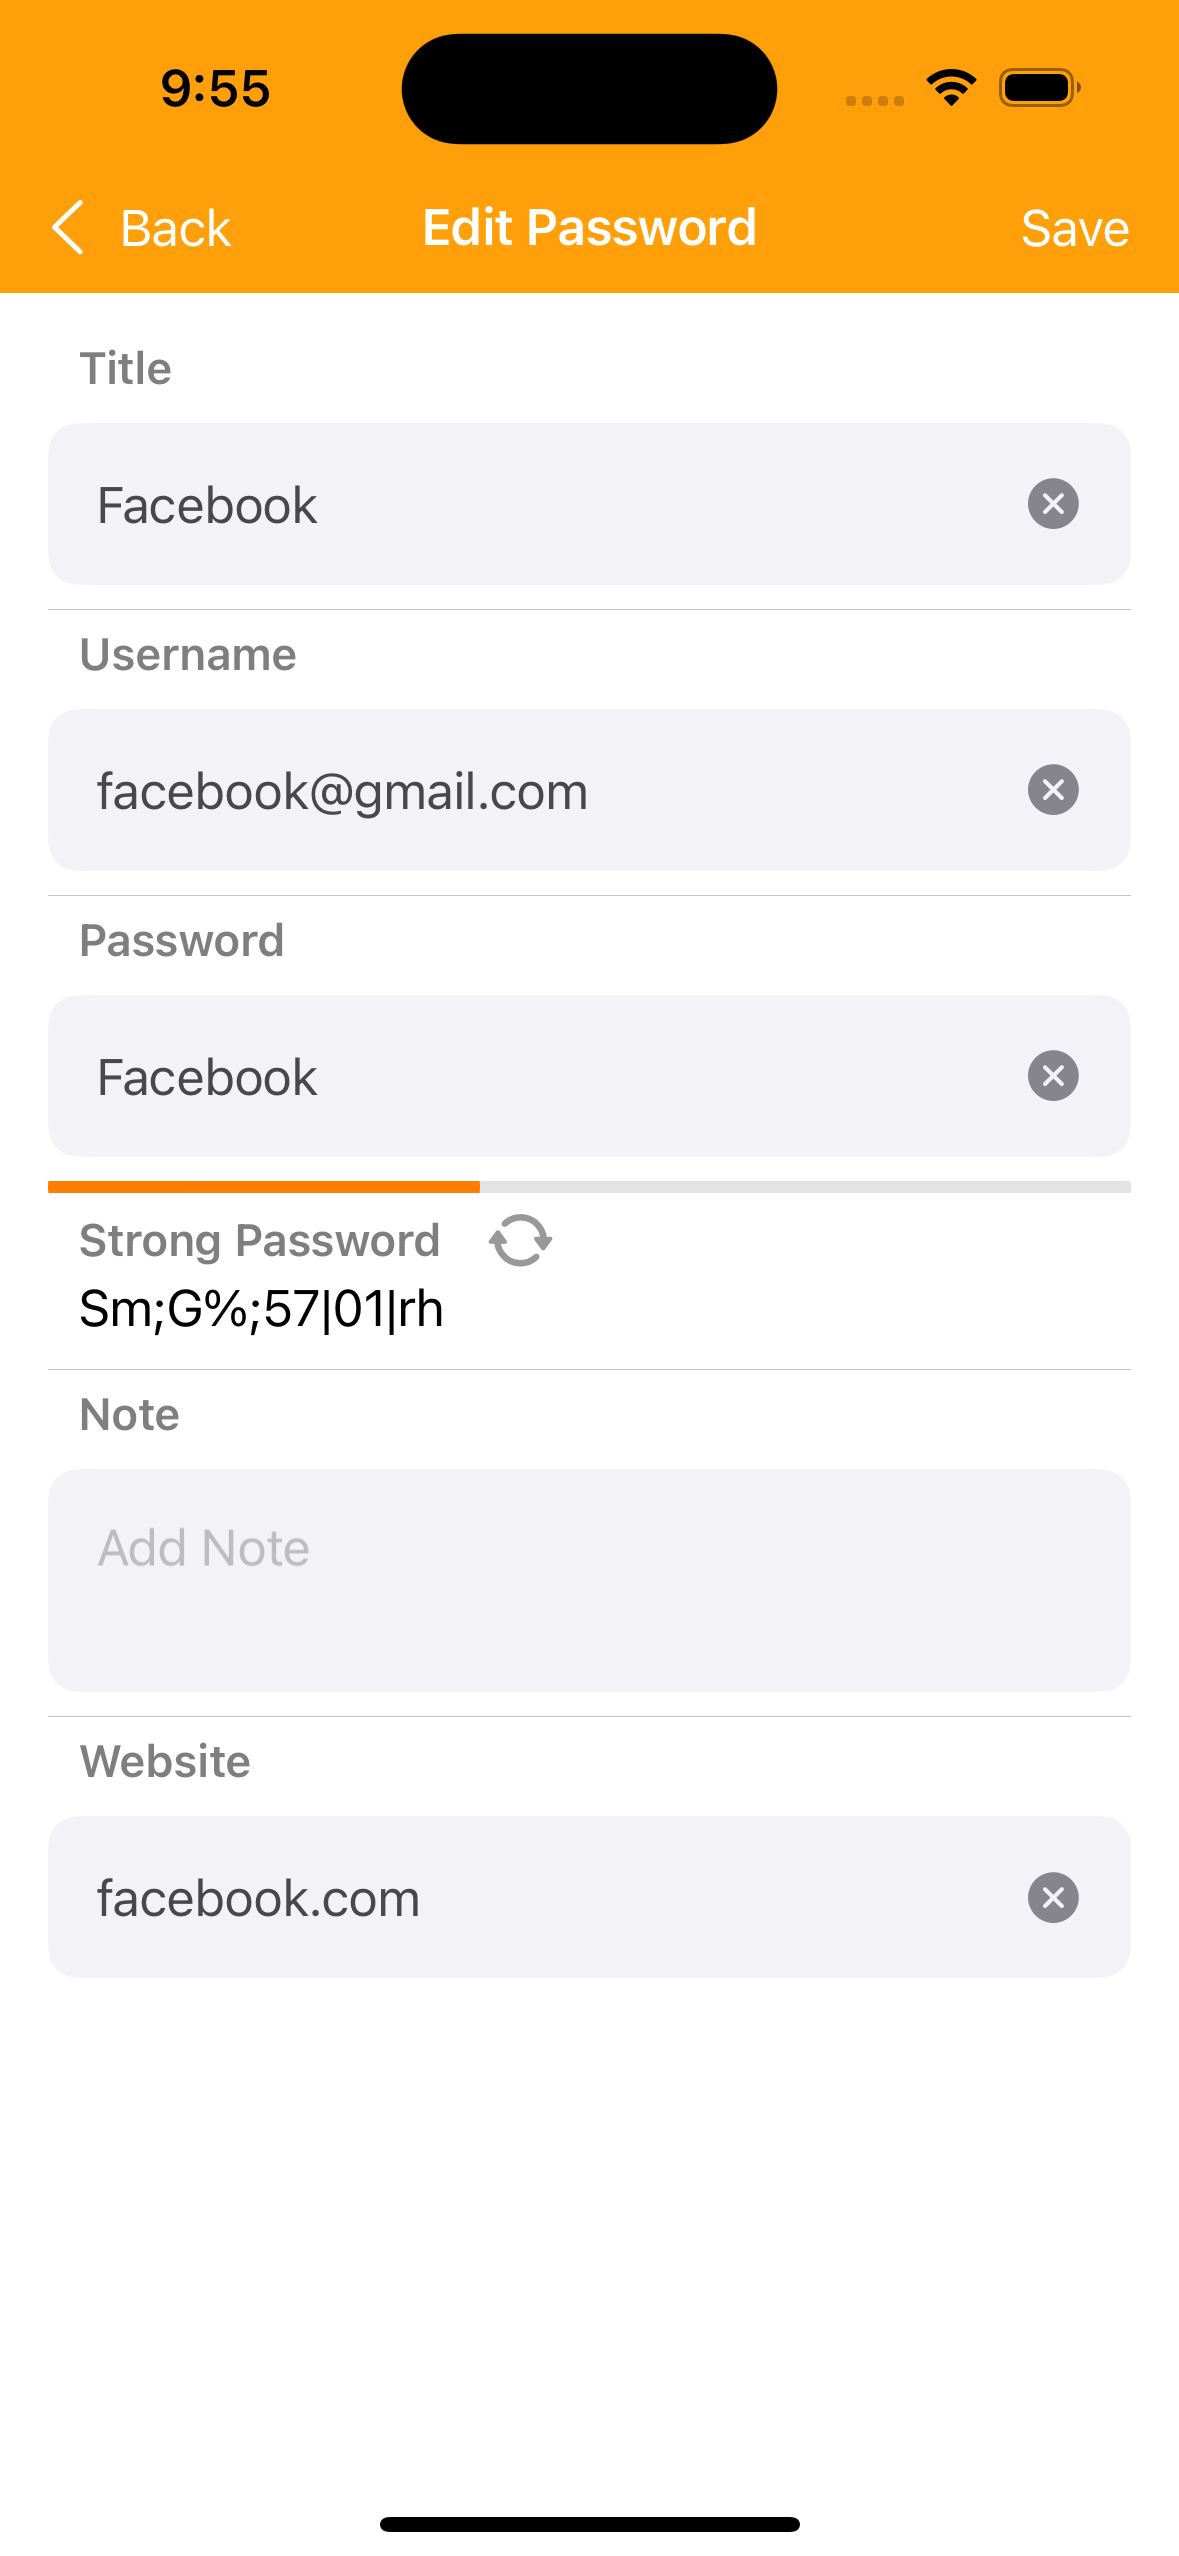
\includegraphics[width=0.3\textwidth]{img/edit_pw}
	\vspace{-0.75em}
	\caption{Editing password}
	\label{fig:edit_pw}
	\vspace{-0.75em}
\end{figure}

This interface mirrors the layout shown in \autoref{fig:add_pw}, with the added convenience that all fields are prepopulated with previously stored data.

\section*{Hash}
\addcontentsline{toc}{section}{Hash}
The master password is securely hashed using the SHA-256 algorithm prior to storage. The following code snippet illustrates this implementation:
\begin{center}
\begin{minipage}{\textwidth}
\begin{lstlisting}
private let saltLength = 16

// set the master password
func setMasterPassword(_ pw: String) {
  // generate salt and save to UserDefault
  let salt = getSalt()
  UserDefaults.standard.set(salt, forKey: saltKey)
  // add salt, hash and save to UserDefault
  UserDefaults.standard.set(hashPassword(pw, salt: salt), 
                            forKey: masterPwKey)
}
  
// generates random data with @saltLength as bite size
private func getSalt() -> Data {
  let salt = Data(count: saltLength)
  var mutableSalt = salt
  _ = mutableSalt.withUnsafeMutableBytes { mutableBytes in
    SecRandomCopyBytes(kSecRandomDefault, saltLength, 
                       mutableBytes.baseAddress!)
  }
  return mutableSalt
}
  
// hash @pw using SHA-256
private func hashPassword(_ pw: String, salt: Data) -> Data {
  // convert string to data
  guard let pwData = pw.data(using: .utf8) else {
    fatalError("Failed to convert password to data")
  }
  // add salt
  let data = pwData + salt
  // hash the password using SHA-256
  return Data(SHA256.hash(data: data))
}
\end{lstlisting}
\end{minipage}
\end{center}

Firstly, the \texttt{setMasterPassword(\_:)} function initiates the process by generating a random salt of 16 bytes in length using the \texttt{getSalt()} method. This salt is then securely stored in the user defaults for future reference. Subsequently, the master password, accompanied by the generated salt, undergoes a hashing procedure via the \texttt{hashPassword(\_:salt:)} function. This function converts the password string into data and concatenates it with the salt before applying the SHA-256 hashing algorithm from \texttt{CryptoKit} framework to generate a hashed representation of the password. The resultant hashed password is then stored securely in the user defaults under a designated key.

The \texttt{getSalt()} function is responsible for generating random data of specified length, serving as the salt for password hashing. It utilizes \texttt{SecRandomCopyBytes} from Apple's Security framework to ensure the creation of cryptographically secure random bytes.

The function that checks if entered password is correct is shown below.
\begin{center}
\begin{minipage}{\linewidth}
\begin{lstlisting}
// checks if master password saved in UserDefaults matches @pw
func doesMasterPasswordMatch(_ pw: String) -> Bool {
  // get master password from UserDefault
  guard let masterPw = UserDefaults.standard.data(forKey: masterPwKey) else {
    return false
  }
  // get salt from UserDefault
  guard let salt = UserDefaults.standard.data(forKey: saltKey) else {
    return false
  }
  // since master password is saved after being hashed
  // compare @pw after adding same salt and hashing
  return hashPassword(pw, salt: salt) == masterPw
}
\end{lstlisting}
\end{minipage}
\end{center}
Firstly, the function retrieves both the hashed master password and its corresponding salt from UserDefaults. If either of these values is absent, indicating that no master password has been previously set, the function immediately returns false, signaling a mismatch.
Next, the function hashes the provided password using the same salt retrieved from UserDefaults and compares the resultant hash with the stored master password. This comparison ensures that the provided password, when processed with the same salt and hashing algorithm used during the initial password setup, matches the stored master password byte-for-byte.

\section*{Encryption}
\addcontentsline{toc}{section}{Encryption}
All passwords are encrypted using the Advanced Encryption Standard (AES) with Galois Counter Mode (GCM), a highly secure encryption method endorsed by prestigious organizations worldwide. AES has become the encryption standard of choice, endorsed by the US Government and numerous prestigious organizations worldwide \cite{team_password}. Hackers can only crack an AES-encrypted password by employing a brute-force attack, attempting various password combinations until they find the correct one. AES-GCM operates with a symmetric key, meaning the same key is used for both encryption and decryption processes. This symmetric key system ensures efficiency and security, as it simplifies the encryption and decryption processes while maintaining robust protection against unauthorized access. 
\begin{center}
\begin{minipage}{\linewidth}
\begin{lstlisting}
private var key = SymmetricKey(size: .bits256)

init() {
  // if the symmetric key has already been generated, assign it to @key
  // otherwise, create new key and save it to UserDefaults
  if let keyData = UserDefaults.standard.data(forKey: symmetricKey) {
    key = SymmetricKey(data: keyData)
  } else {
    // new symmetric key is created when object of this class is created
    // convert symmetric key to Data and store in UserDefaults
    let keyData = key.withUnsafeBytes { Data($0) }
    UserDefaults.standard.set(keyData, forKey: symmetricKey)
  }
}
\end{lstlisting}
\end{minipage}
\end{center}
It begins by defining constant \texttt{symmetricKey} to hold the identifier for storing and retrieving the key from user defaults and initializing symmetric key using \texttt{SymmetricKey(size:.bits256)} which creates a symmetric key with 256 bits. 

Within the \texttt{init()} method, it attempts to retrieve the symmetric key stored in the user defaults under the identifier \texttt{symmetricKey}. If the key data is found, it is used to initialize \texttt{key} variable. Otherwise, key has not been generated yet, so convert key generated in line 1 into a \texttt{Data} object and stored in the user defaults under the \texttt{symmetricKey} identifier for future use. When adding a new password or changing existing password, this \texttt{key} is used to encrypt.

\begin{center}
\begin{minipage}{\linewidth}
\begin{lstlisting}
// add @pw to the database after encrypting its password
func addPassword(_ pw: Password, context: NSManagedObjectContext) {
  // encrypt password
  guard let password = encrypt(pw.password) else { return }
  // save to database
  DataController().addPassword(title: pw.title,
                               username: pw.username,
                               password: password,
                               note: pw.note,
                               website: pw.website,
                               context: context)
}

// edit @pw in the database after encrypting its password
func editPassword(_ pw: Password, to passwords: Passwords, 
                    context: NSManagedObjectContext) {
  // encrypt password
  guard let password = encrypt(pw.password) else { return }
  // save to database
  DataController().editPassword(passwords,
                                title: pw.title,
                                username: pw.username,
                                password: password,
                                note: pw.note,
                                website: pw.website,
                                context: context)
}
\end{lstlisting}
\end{minipage}
\end{center}
When adding or editing the password, password is encrypted before storage. This process ensures that sensitive user information remains protected against unauthorized access. The code for encryption is shown below. 
\begin{center}
\begin{minipage}{\linewidth}
\begin{lstlisting}
// encrypts @pw and return encrypted password as Data
private func encrypt(_ pw: String) -> Data? {
  // convert string to data before encryption
  guard let pwData = pw.data(using: .utf8) else {
    return nil
  }
  // add salt
  let data = pwData + getSalt()
  do {
    let sealedBox = try AES.GCM.seal(data, using: key)
    return sealedBox.combined
  } catch {
    print("Encryption failed: \(error.localizedDescription)")
    return nil
  }
}
\end{lstlisting}
\end{minipage}
\end{center}
The encryption process begins by converting the plaintext password into a \texttt{Data} object using UTF-8 encoding. This step ensures that the password is in a format suitable for cryptographic operations. It then incorporates a salt to enhance the security of the encryption process.

Within a do-catch block, the encryption attempts to use the \texttt{AES.GCM.seal} method, which seals the plaintext data using the provided encryption key, \texttt{key}. If successful, the encrypted data is encapsulated within a sealed box. Finally, the combined ciphertext and authentication tag are extracted from the sealed box and returned as Data.

\begin{center}
\begin{minipage}{\linewidth}
\begin{lstlisting}
// decrypts @encryptedData and return the original password as string
func getPassword(_ encryptedData: Data) -> String {
  return decryptPassword(encryptedData) ?? ""
}

// decrypts @encryptedData and return password as string
private func decryptPassword(_ encryptedData: Data) -> String? {
  do {
    // decrypts using AES-GCM algorithm
    let sealedBox = try AES.GCM.SealedBox(combined: encryptedData)
    let decryptedData = try AES.GCM.open(sealedBox, using: key)
    // extract salt from decrypted data
    let pwData = decryptedData.dropLast(saltLength)
    // converts data to string using UTF8
    return String(data: pwData, encoding: .utf8)
  } catch {
    print("Decryption failed: \(error.localizedDescription)")
    return nil
  }
}
\end{lstlisting}
\end{minipage}
\end{center}
When displaying the password, the program needs to decrypt the saved password. The function, \texttt{decryptPassword} uses same symmetric key to decrypt. The encrypted data is first encapsulated within a sealed box using the AES-GCM algorithm. This sealed box is then passed to the \texttt{AES.GCM.open} method along with the symmetric key. If successful, the decrypted data is obtained, salt is extracted and it is converted back to a string using UTF-8 encoding.

\section*{Conclusion}
\addcontentsline{toc}{section}{Conclusion}
The password manager app developed in Swift ensures robust security for managing passwords. It employs advanced encryption and hashing techniques, including SHA-256 for hashing master password and AES-GCM algorithm for encrypting and decrypting passwords. By prioritizing both security and convenience, the app addresses the crucial need for safeguarding sensitive data.

\newpage
\bibliographystyle{IEEEtran}
\bibliography{references}

\end{document}